

\documentclass[a4paper]{article}

\usepackage[english]{babel}
\usepackage{amsmath}
\usepackage{tikz}
\usepackage{listings}
\usepackage{pxfonts}
\usepackage[margin=1in]{geometry}
\usepackage[nottoc]{tocbibind}
\usepackage{xcolor}
\usepackage{float}

\setcounter{MaxMatrixCols}{12}
\usetikzlibrary{arrows.meta,calc}
\tikzset{>={Latex[width=1.2mm,length=2.5mm]}}
\lstset{
	belowcaptionskip=1\baselineskip,
	breaklines=true,
	xleftmargin=\parindent,
	language=C++,
	showstringspaces=false,
	basicstyle=\ttfamily\small,
	keywordstyle=\bfseries\color{green!40!black},
	commentstyle=\itshape\color{purple!40!black},
	identifierstyle=\color{blue},
	stringstyle=\color{orange},
	tabsize=2,
}


\title{The Finite Element Method by Example in Qt/C++}
\author{Krzysztof Napiontek\protect\\knapiontek@gmail.com}
\date{Version 1.0\protect\\\today}

\begin{document}

\maketitle

\begin{abstract}

The aim of this article is help with understanding The Finite Element Method in mechanics. The theoretical part is reduced to its minimum and most of the work is focused on diagrams, graphics and examples. The relevant part of source code calculating tetrahedron truss is presented at the end of each section along with its visualized output.

\end{abstract}

\tableofcontents

\pagebreak

\section{Introduction}

There are many works presenting FEM, most of them very complex and comprehensive with purpose of full explanation of all details of the method. A reader who needs explanation of general idea behind finds it difficult to understand. This work tries to extract the most important aspects in a way helping to understand all knowledge almost at the first read. The relevant source code added at the end of each section calculates and visualizes the simplest 3D truss object - tetrahedron. The Hook's Law is the only equation borrowed from mechanics. There is also a need to understand trigonometry and basic matrix operations before reading.

\section{The Concrete Example}

For the purpose of this article the complete concrete example was implemented. It includes data type definitions, construction of a matrix equation, its solution and in final the presentation in graphics format. A number of dumps of the equation data have been generated for better understanding parts of implementation. The source code presented in this work was tested with Qt 5.1 in Windows environment. It does not use any platform specific code and can be easily ported to other systems.

\bigskip

The final result of the example is presented on the figure \ref{fig:final:graphics}. It contains an original geometry of the truss, also geometry deformation by an external force and reactions in fixed points. Detailed explanation will be given in following chapters.

\begin{figure}[H]
\centering
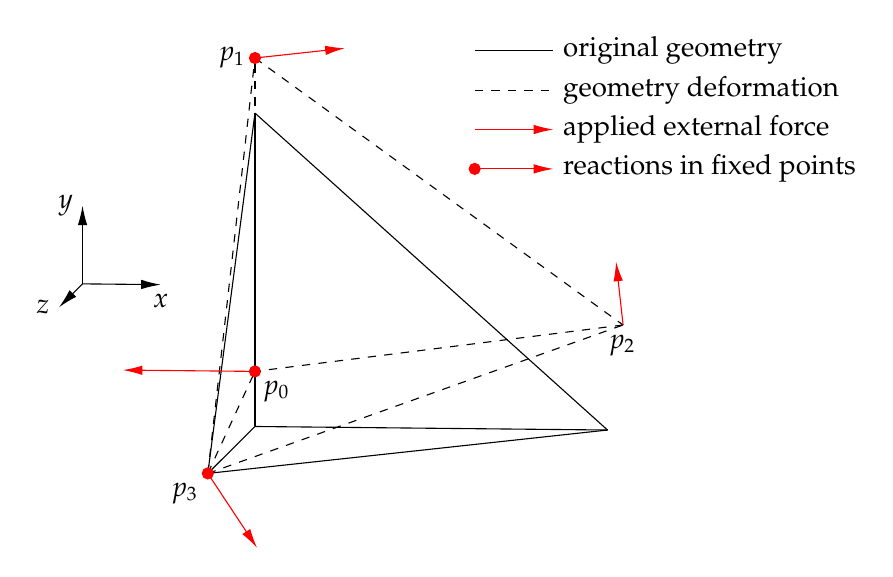
\begin{tikzpicture}
\draw[->] (-0.980017,2.03987) -- (0.0149875,2.0299);
\node[below] at (0.0149875,2.0299) {$x$};
\draw[->] (-0.980017,2.03987) -- (-0.980017,3.03487);
\node[left] at (-0.980017,3.03487) {$y$};
\draw[->] (-0.980017,2.03987) -- (-1.27952,1.74186);
\node[left] at (-1.27952,1.74186) {$z$};
\draw (1.20966,0.228594) -- (1.20966,4.20861);
\draw (1.20966,4.20861) -- (5.68718,0.183744);
\draw (5.68718,0.183744) -- (1.20966,0.228594);
\draw (0.610658,-0.367414) -- (1.20966,0.228594);
\draw (0.610658,-0.367414) -- (1.20966,4.20861);
\draw (0.610658,-0.367414) -- (5.68718,0.183744);
\draw[dashed] (1.20966,0.928164) -- (1.20966,4.90818);
\draw[dashed] (1.20966,4.90818) -- (5.88499,1.51754);
\draw[dashed] (5.88499,1.51754) -- (1.20966,0.928164);
\draw[dashed] (0.610658,-0.367414) -- (1.20966,0.928164);
\draw[dashed] (0.610658,-0.367414) -- (1.20966,4.90818);
\draw[dashed] (0.610658,-0.367414) -- (5.88499,1.51754);
\draw[fill,red] (1.20966,0.928164) circle(0.07);
\draw[->,red] (1.20966,0.928164) -- (-0.469411,0.944983);
\node[below right] at (1.20966,0.928164) {$p_0$};
\draw[fill,red] (1.20966,4.90818) circle(0.07);
\draw[->,red] (1.20966,4.90818) -- (2.35188,5.03219);
\node[left] at (1.20966,4.90818) {$p_1$};
\draw[->,red] (5.88499,1.51754) -- (5.79514,2.32364);
\node[below] at (5.88499,1.51754) {$p_2$};
\draw[fill,red] (0.610658,-0.367414) circle(0.07);
\draw[->,red] (0.610658,-0.367414) -- (1.23736,-1.31435);
\node[below left] at (0.610658,-0.367414) {$p_3$};
\draw (4,5) -- (5,5);
\node[right] at (5,5) {original geometry};
\draw[dashed] (4,4.5) -- (5,4.5);
\node[right] at (5,4.5) {geometry deformation};
\draw[->,red] (4,4) -- (5,4);
\node[right] at (5,4) {applied external force};
\draw[->,red] (4,3.5) -- (5,3.5);
\node[right] at (5,3.5) {reactions in fixed points};
\draw[fill,red] (4,3.5) circle(0.07);
\end{tikzpicture}
\caption{The Graphics Generated by the Example}
\label{fig:final:graphics}
\end{figure}

\subsection{Global Data Definition in the Example}

\lstinputlisting{data.cpp}

\section{The Finite Element Method}

The FEM analyse in this chapter finds relation between forces and displacements in global coordinates. At first it breaks down the truss into separate elements, finds relation of them in local coordinates using the Hook's Law and in next step it transforms it to global coordinate system for each element. Finally it aggregates all elements in one global matrix of stiffness. The lower case bold font is reserved for local and the upper case bold font for global matrices and vectors.

\subsection{Tetrahedron Truss Breakdown}

The first step of analyses requires the truss breakdown. Each element will be analysed separately and finally all of them will be aggregated in global matrix. Separation of elements is shown on the figure \ref{fig:breakdown}.

\begin{figure}[H]
\centering
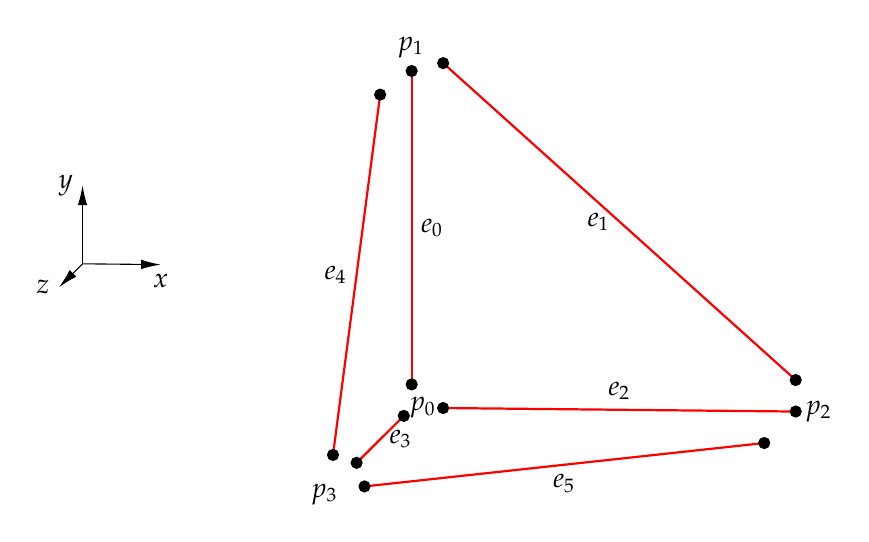
\begin{tikzpicture}
\draw[->] (-2.97002,2.0598) -- (-1.97502,2.04983);
\node[below] at (-1.97502,2.04983) {$x$};
\draw[->] (-2.97002,2.0598) -- (-2.97002,3.0548);
\node[left] at (-2.97002,3.0548) {$y$};
\draw[->] (-2.97002,2.0598) -- (-3.26953,1.7618);
\node[left] at (-3.26953,1.7618) {$z$};
\draw[thick,red] (1.20966,0.528594) -- (1.20966,4.50861);
\draw[fill] (1.20966,0.528594) circle(0.07);
\draw[fill] (1.20966,4.50861) circle(0.07);
\node[right] at (1.20966,2.5186) {$e_0$};
\draw[thick,red] (1.60966,4.60861) -- (6.08718,0.583744);
\draw[fill] (1.60966,4.60861) circle(0.07);
\draw[fill] (6.08718,0.583744) circle(0.07);
\node[left] at (3.84842,2.59618) {$e_1$};
\draw[thick,red] (6.08718,0.183744) -- (1.60966,0.228594);
\draw[fill] (6.08718,0.183744) circle(0.07);
\draw[fill] (1.60966,0.228594) circle(0.07);
\node[above] at (3.84842,0.206169) {$e_2$};
\draw[thick,red] (0.510658,-0.467414) -- (1.10966,0.128594);
\draw[fill] (0.510658,-0.467414) circle(0.07);
\draw[fill] (1.10966,0.128594) circle(0.07);
\node[right] at (0.810158,-0.16941) {$e_3$};
\draw[thick,red] (0.210658,-0.367414) -- (0.809659,4.20861);
\draw[fill] (0.210658,-0.367414) circle(0.07);
\draw[fill] (0.809659,4.20861) circle(0.07);
\node[left] at (0.510158,1.9206) {$e_4$};
\draw[thick,red] (0.610658,-0.767414) -- (5.68718,-0.216256);
\draw[fill] (0.610658,-0.767414) circle(0.07);
\draw[fill] (5.68718,-0.216256) circle(0.07);
\node[below] at (3.14892,-0.491835) {$e_5$};
\node at (1.35966,0.228594) {$p_0$};
\node at (1.20966,4.80861) {$p_1$};
\node at (6.38718,0.183744) {$p_2$};
\node at (0.110658,-0.867414) {$p_3$};
\end{tikzpicture}
\caption{Truss Breakdown}
\label{fig:breakdown}
\end{figure}

\subsection{The Stiffness Matrix of an Element in Local Coordinates}

Relation between axial forces $f_0, f_1$ and axial displacements $\Delta p_0, \Delta p_1$ in local coordinates in respect of the Hook's Law as depicted on the figure \ref{fig:displacement:and:force} is described by equations \ref{eq:hook0} and \ref{eq:hook1} . Despite of 3D analyses most of the figures use 2D coordinates for simplicity.

\begin{equation}
f_0 = \frac {EA} L (\Delta p_0 - \Delta p_1)
\label{eq:hook0}
\end{equation}
\begin{equation}
f_1 = \frac {EA} L (\Delta p_1 - \Delta p_0)
\label{eq:hook1}
\end{equation}

\begin{figure}[H]
\centering
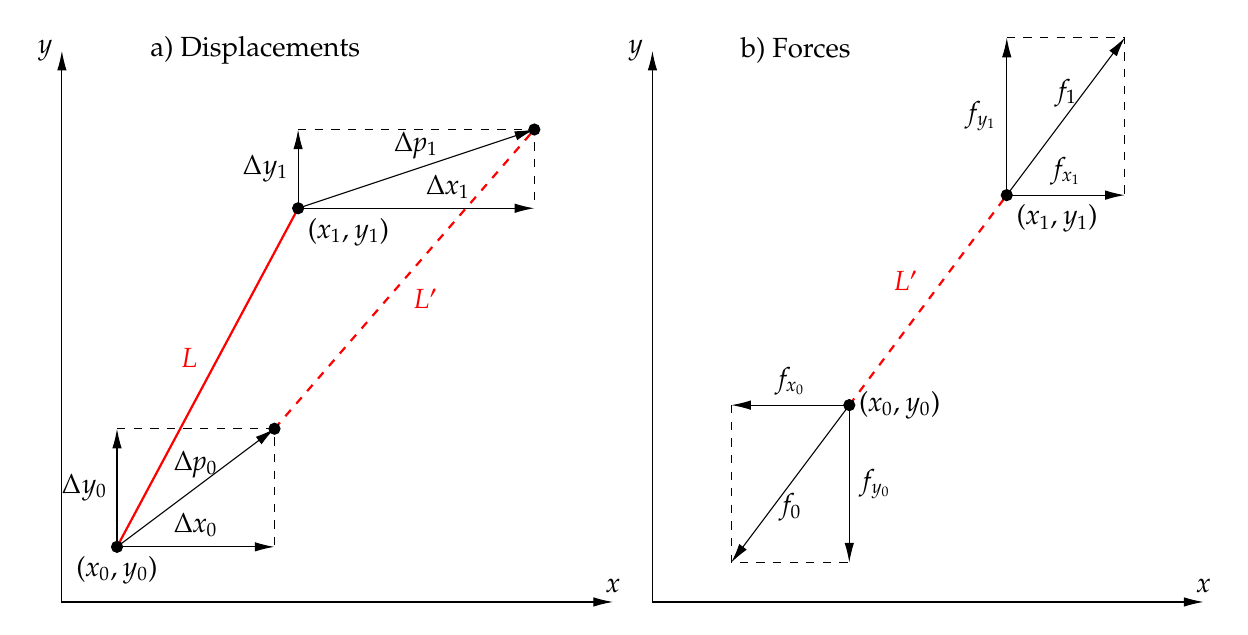
\begin{tikzpicture}
\node[right] at (1,7) {a) Displacements};
\draw[<->] (0,7) -- (0,0) -- (7,0);
\node[above] at (7,0) {$x$};
\node[left] at (0,7) {$y$};
\draw[dashed] (0.7,2.2) -- (2.7,2.2) -- (2.7,0.7);
\draw[<->] (0.7,2.2) -- (0.7,0.7) -- (2.7,0.7);
\node[above] at (1.7,0.7) {$\Delta x_0$};
\node[left] at (0.7,1.45) {$\Delta y_0$};
\draw[->] (0.7,0.7) -- (2.7,2.2);
\node[above] at (1.7,1.45) {$\Delta p_0$};
\node[below] at (0.7,0.7) {$(x_0,y_0)$};
\draw[dashed] (3,6) -- (6,6) -- (6,5);
\draw[<->] (3,6) -- (3,5) -- (6,5);
\node[above right] at (4.5,5) {$\Delta x_1$};
\node[left] at (3,5.5) {$\Delta y_1$};
\draw[->] (3,5) -- (6,6);
\node[above] at (4.5,5.5) {$\Delta p_1$};
\node[below right] at (3,5) {$(x_1,y_1)$};
\draw[thick,red] (0.7,0.7) -- (3,5);
\node[thick,red,above left] at (1.85,2.85) {$L$};
\draw[fill] (0.7,0.7) circle(0.07);
\draw[fill] (3,5) circle(0.07);
\draw[thick,dashed,red] (2.7,2.2) -- (6,6);
\node[red,below right] at (4.35,4.1) {$L'$};
\draw[fill] (2.7,2.2) circle(0.07);
\draw[fill] (6,6) circle(0.07);
\node[right] at (8.5,7) {b) Forces};
\draw[<->] (7.5,7) -- (7.5,0) -- (14.5,0);
\node[above] at (14.5,0) {$x$};
\node[left] at (7.5,7) {$y$};
\draw[dashed] (8.5,2.5) -- (8.5,0.5) -- (10,0.5);
\draw[<->] (8.5,2.5) -- (10,2.5) -- (10,0.5);
\node[above] at (9.25,2.5) {$f_{x_0}$};
\node[right] at (10,1.5) {$f_{y_0}$};
\draw[->] (10,2.5) -- (8.5,0.5);
\node[below] at (9.25,1.5) {$f_0$};
\node[right] at (10,2.5) {$(x_0,y_0)$};
\draw[dashed] (12,7.16667) -- (13.5,7.16667) -- (13.5,5.16667);
\draw[<->] (12,7.16667) -- (12,5.16667) -- (13.5,5.16667);
\node[above] at (12.75,5.16667) {$f_{x_1}$};
\node[left] at (12,6.16667) {$f_{y_1}$};
\draw[->] (12,5.16667) -- (13.5,7.16667);
\node[above] at (12.75,6.16667) {$f_1$};
\node[below right] at (12,5.16667) {$(x_1,y_1)$};
\draw[thick,dashed,red] (10,2.5) -- (12,5.16667);
\node[red,above left] at (11,3.83333) {$L'$};
\draw[fill] (10,2.5) circle(0.07);
\draw[fill] (12,5.16667) circle(0.07);
\end{tikzpicture}
\caption{Displacements (a) and Stress Forces (b) in an Element}
\label{fig:displacement:and:force}
\end{figure}

In fact the method provides only approximated solution since it assumes that angles between elements stay the same after applying external forces. In reality such approach is accepted   as long as deformations are small.

\bigskip

Using matrix notation we isolate local stiffness matrix $\mathbf{k}$.

\begin{equation}
\begin{bmatrix}
	f_0 \\
	f_1
\end{bmatrix}
= \frac {EA} L
\begin{bmatrix}
	1 & -1 \\
	-1 & 1
\end{bmatrix}
\begin{bmatrix}
	\Delta p_0 \\
	\Delta p_1
\end{bmatrix}
\end{equation}

\begin{equation}
\mathbf k = \frac {EA} L
\begin{bmatrix}
	1 & -1 \\
	-1 & 1
\end{bmatrix}
\end{equation}

The stiffness matrix represents geometry in an algebraic form. Final form of matrix equation in local coordinates shown below. Lower case bold letters reserved for local coordinates.

\begin{equation}
\mathbf{f} = \mathbf{k} \Delta \mathbf{p}
\end{equation}

\subsection{Coordinate Transformation}

In previous chapter we described relations in local coordinates. In order to aggregate all elements into global system a number of transformations have to take place.

\subsubsection{Global and Local Coordinates Relations}

The figure \ref{fig:displacement:and:force}a can be used in order to describe local and global geometrical relations.

\begin{equation}
L = \sqrt { (x_1 - x_0)^2 + (y_1 - y_0)^2 + (z_1 - z_0)^2 }
\end{equation}
\begin{equation}
c_x = \cos \theta_x = \frac {x_1 - x_0} L
\end{equation}
\begin{equation}
c_y = \cos \theta_y = \frac {y_1 - y_0} L
\end{equation}
\begin{equation}
c_z = \cos \theta_z = \frac {z_1 - z_0} L
\end{equation}

\subsubsection{The Point Displacement Relations}

The displacement from the figure \ref{fig:displacement:and:force}a for the point $p_0$ is broken down on the figure \ref{fig:displacement:details}.

\begin{figure}[H]
\centering
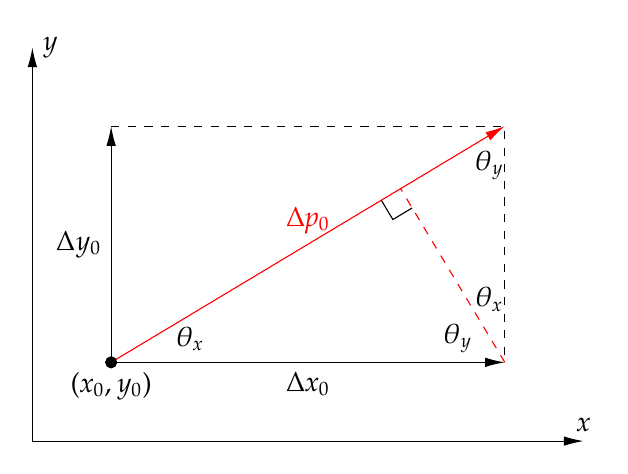
\begin{tikzpicture}
\draw[<->] (0,5) -- (0,0) -- (7,0);
\node[above] at (7,0) {$x$};
\node[right] at (0,5) {$y$};
\draw[dashed] (1,4) -- (6,4) -- (6,1);
\draw[<->] (1,4) -- (1,1) -- (6,1);
\node[below] at (3.5,1) {$\Delta x_0$};
\node[left] at (1,2.5) {$\Delta y_0$};
\draw[->,red] (1,1) -- (6,4);
\node[red,above] at (3.5,2.5) {$\Delta p_0$};
\draw[dashed,red] (6,1) -- (4.67647,3.20588);
\node at (2,1.3) {$\theta_x$};
\node at (5.4,1.3) {$\theta_y$};
\node at (5.8,1.8) {$\theta_x$};
\node at (5.8,3.5) {$\theta_y$};
\draw[fill] (1,1) circle(0.07);
\node[below] at (1,1) {$(x_0,y_0)$};
\draw (4.43137,3.05882) -- (4.57843,2.81373) -- (4.82353,2.96078);
\end{tikzpicture}
\caption{Displacement of the Point $p_0$ in Details}
\label{fig:displacement:details}
\end{figure}

From congruence of triangles as on the figure \ref{fig:displacement:details} we obtain

\begin{equation}
\Delta p_0 = \Delta x_0 \cos \theta_x + \Delta y_0 \cos \theta_y + \Delta z_0 \cos \theta_z
\end{equation}
\begin{equation}
\Delta p_1 = \Delta x_1 \cos \theta_x + \Delta y_1 \cos \theta_y + \Delta z_1 \cos \theta_z
\end{equation}

In other words

\begin{equation}
\begin{bmatrix}
	\Delta p_0 \\
	\Delta p_1
\end{bmatrix}
=
\begin{bmatrix}
	c_x & c_y & c_z & 0 & 0 & 0 \\
	0 & 0 & 0 & c_x & c_y & c_z
\end{bmatrix}
\begin{bmatrix}
	\Delta x_0 \\
	\Delta y_0 \\
	\Delta z_0 \\
	\Delta x_1 \\
	\Delta y_1 \\
	\Delta z_1
\end{bmatrix}
\end{equation}

or simpler

\begin{equation}
\Delta \mathbf{p} = \mathbf{T} \Delta \mathbf{P}
\label{eq:displacement:local:vs:global}
\end{equation}

The equation \ref{eq:displacement:local:vs:global} describes displacement relation between local and global coordinates.

\subsubsection{Global and Local Forces Relations}

Forces given directly from geometry on the figure \ref{fig:displacement:and:force}b

\begin{equation}
f_{x_0} = f_0 \cos \theta_x
\end{equation}
\begin{equation}
f_{y_0} = f_0 \cos \theta_y
\end{equation}
\begin{equation}
f_{z_0} = f_0 \cos \theta_z
\end{equation}
\begin{equation}
f_{x_1} = f_1 \cos \theta_x
\end{equation}
\begin{equation}
f_{y_1} = f_1 \cos \theta_y
\end{equation}
\begin{equation}
f_{z_1} = f_1 \cos \theta_z
\end{equation}

or in a matrix form

\begin{equation}
\begin{bmatrix}
	f_{x_0} \\
	f_{y_0} \\
	f_{z_0} \\
	f_{x_1} \\
	f_{y_1} \\
	f_{z_1}
\end{bmatrix}
=
\begin{bmatrix}
	c_x & 0 \\
	c_y & 0 \\
	c_z & 0 \\
	0 & c_x \\
	0 & c_y \\
	0 & c_z
\end{bmatrix}
\begin{bmatrix}
	f_0 \\
	f_1
\end{bmatrix}
\end{equation}

\begin{equation}
\mathbf{F = T^T f}
\label{eq:forces:local:vs:global}
\end{equation}

The equation \ref{eq:forces:local:vs:global} describes forces relation between local and global coordinates.

\subsection{The Stiffness Matrix of an Element in Global Coordinates}

Equations obtained in previous chapter: Hook's law, displacement and force relations between local and global coordinates are repeated below.

\begin{equation}
\mathbf{f} = \mathbf{k} \Delta \mathbf{p}
\end{equation}
\begin{equation}
\Delta \mathbf{p} = \mathbf{T} \Delta \mathbf{P}
\end{equation}
\begin{equation}
\mathbf{F = T^T f}
\end{equation}

It can be transformed into

\begin{equation}
\mathbf{f} = \mathbf{k} \Delta \mathbf{p}
\end{equation}
\begin{equation}
\mathbf{f} = \mathbf{k T} \Delta \mathbf{P}
\end{equation}
\begin{equation}
\mathbf{T^T f} = \mathbf{T^T k T} \Delta \mathbf{P}
\end{equation}
\begin{equation}
\mathbf{F} = \mathbf{T^T k T} \Delta \mathbf{P}
\end{equation}

Finally the extracted version of global stiffness matrix $\mathbf{K}$ in global coordinates takes form

\begin{equation}
\mathbf{K} = \mathbf{T^T k T} = \frac {EA} L
\begin{bmatrix}
	c^2_x & c_xc_y & c_xc_z & -c^2_x & -c_xc_y & -c_xc_z \\
	c_xc_y & c^2_y & c_yc_z & -c_xc_y & -c^2_y & -c_yc_z \\
	c_xc_z & c_yc_z & c^2_z & -c_xc_z & -c_yc_z & -c^2_z \\
	-c^2_x & -c_xc_y & -c_xc_z & c^2_x & c_xc_y & c_xc_z \\
	-c_xc_y & -c^2_y & -c_yc_z & c_xc_y & c^2_y & c_yc_z \\
	-c_xc_z & -c_yc_z & -c^2_z & c_xc_z & c_yc_z & c^2_z
\end{bmatrix}
\end{equation}

so the main equation of this work is formed as

\begin{equation}
\mathbf{F} = \mathbf{K} \Delta \mathbf{P}
\label{eq:main}
\end{equation}

and describes relation of global forces and deformation of whole truss geometry.

\subsection{Global Stiffness Matrix Aggregation}

Let's form equation \ref{eq:main} for an element $e_2(p_0,p_2)$ in Global Stiffness Matrix. The element index for cosines is omitted for simplicity ($c_x$ instead of $c_{2_x}$ etc.).

\begin{equation}
\frac {EA} L
\begin{bmatrix}
	c^2_x & c_xc_y & c_xc_z & . & . & . & -c^2_x & -c_xc_y & -c_xc_z & . & . & . \\
	c_xc_y & c^2_y & c_yc_z & . & . & . & -c_xc_y & -c^2_y & -c_yc_z & . & . & . \\
	c_xc_z & c_yc_z & c^2_z & . & . & . & -c_xc_z & -c_yc_z & -c^2_z & . & . & . \\
	. & . & . & . & . & . & . & . & . & . & . & . \\
	. & . & . & . & . & . & . & . & . & . & . & . \\
	. & . & . & . & . & . & . & . & . & . & . & . \\
	-c^2_x & -c_xc_y & -c_xc_z & . & . & . & c^2_x & c_xc_y & c_xc_z & . & . & . \\
	-c_xc_y & -c^2_y & -c_yc_z & . & . & . & c_xc_y & c^2_y & c_yc_z & . & . & . \\
	-c_xc_z & -c_yc_z & -c^2_z & . & . & . & c_xc_z & c_yc_z & c^2_z & . & . & . \\
	. & . & . & . & . & . & . & . & . & . & . & . \\
	. & . & . & . & . & . & . & . & . & . & . & . \\
	. & . & . & . & . & . & . & . & . & . & . & .
\end{bmatrix}
\begin{bmatrix}
	\Delta x_0 \\
	\Delta y_0 \\
	\Delta z_0 \\
	. \\
	. \\
	. \\
	\Delta x_2 \\
	\Delta y_2 \\
	\Delta z_2 \\
	. \\
	. \\
	.
\end{bmatrix}
=
\begin{bmatrix}
	f_{x_0} \\
	f_{y_0} \\
	f_{z_0} \\
	. \\
	. \\
	. \\
	f_{x_2} \\
	f_{y_2} \\
	f_{z_2} \\
	. \\
	. \\
	.
\end{bmatrix}
\label{eq:detail:K:element}
\end{equation}

By substituting parts of above equation by

\begin{equation}
k_2 = \frac {EA} L
\begin{bmatrix}
	c^2_x & c_xc_y & c_xc_z \\
	c_xc_y & c^2_y & c_yc_z \\
	c_xc_z & c_yc_z & c^2_z
\end{bmatrix}
\;\;\;\;\;
\Delta p_i =
\begin{bmatrix}
	\Delta x_i \\
	\Delta y_i \\
	\Delta z_i
\end{bmatrix}
\;\;\;\;\;
f_i =
\begin{bmatrix}
	f_{x_i} \\
	f_{y_i} \\
	f_{z_i}
\end{bmatrix}
\end{equation}

we obtain simpler form ready for further analysis

\begin{equation}
\begin{bmatrix}
	k_2 & . & -k_2 & . \\
	. & . & . & . \\
	-k_2 & . & k_2 & . \\
	. & . & . & .
\end{bmatrix}
\begin{bmatrix}
	\Delta p_0 \\
	. \\
	\Delta p_2 \\
	.
\end{bmatrix}
=
\begin{bmatrix}
	f_0 \\
	. \\
	f_2 \\
	.
\end{bmatrix}
\end{equation}

\begin{equation}
\mathbf{K_2} \Delta \mathbf{P} = \mathbf{F_2}
\end{equation}

The sum of all directional forces based on the condition of equilibrium in a point is equal zero

\begin{equation}
\sum \mathbf{F_x} = 0\;\;\;\;\;\sum \mathbf{F_y} = 0\;\;\;\;\;\sum \mathbf{F_z} = 0
\end{equation}

\begin{figure}[H]
\centering
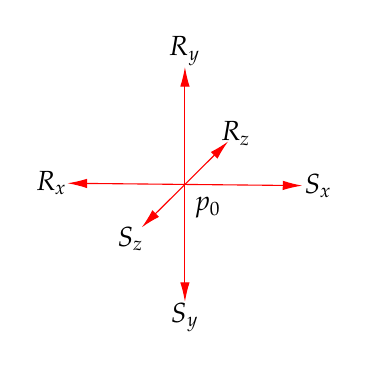
\begin{tikzpicture}
\draw[<->,red] (1.50749,2.01495) -- (4.49251,1.98505);
\node at (1.30749,2.01495) {$R_x$};
\node at (4.69251,1.98505) {$S_x$};
\draw[<->,red] (3,3.49251) -- (3,0.507494);
\node at (3,3.69251) {$R_y$};
\node at (3,0.307494) {$S_y$};
\draw[<->,red] (3.54908,2.54634) -- (2.45092,1.45366);
\node at (3.64908,2.64634) {$R_z$};
\node at (2.31092,1.31366) {$S_z$};
\node at (3.3,1.7) {$p_0$};
\end{tikzpicture}
\caption{Force Equilibrium in the Point $p_0$, \textbf{R}eactions and \textbf{S}tresses}
\label{fig:point0:forces}
\end{figure}

and displacement in the point is the same for all elements based on it. So we can write down

\begin{equation}
\sum\limits_{e=1}^n \mathbf{K_e} \Delta \mathbf{P} = \sum\limits_{e=1}^n \mathbf{F_e}\;\;\;\;\;\mbox{e - index of an element}
\end{equation}

Finally the simplified form of $\mathbf{K}$ for all elements (aggregation with collocation)

\begin{equation}
\begin{bmatrix}
	k_0 + \color{green}{k_2} + \color{blue}{k_3} & -k_0 & \color{green}{-k_2} & \color{blue}{-k_3} \\
	-k_0 & k_0 + \color{red}{k_1} + \color{cyan}{k_4} & \color{red}{-k_1} & \color{cyan}{-k_4} \\
	\color{green}{-k_2} & \color{red}{-k_1} & \color{red}{k_1} + \color{green}{k_2} + k_5 & -k_5 \\
	\color{blue}{-k_3} & \color{cyan}{-k_4} & -k_5 & \color{blue}{k_3} + \color{cyan}{k_4} + k_5
\end{bmatrix}
\begin{bmatrix}
	\Delta p_0 \\
	\Delta p_1 \\
	\Delta p_2 \\
	\Delta p_3
\end{bmatrix}
=
\begin{bmatrix}
	f_0 \\
	f_1 \\
	f_2 \\
	f_3
\end{bmatrix}
\end{equation}

The aggregated version of equation \ref{eq:detail:K:element} is omitted here due to a poor readability.

\bigskip

The numerical version of the stiffness matrix with no forces applied as generated by the concrete example

\begin{equation}
\resizebox{.93 \textwidth}{!} {$
\begin{bmatrix}
222.2 & . & . & . & . & . & -222.2 & . & . & . & . & . \\
. & 250 & . & . & -250 & . & . & . & . & . & . & . \\
. & . & 166.7 & . & . & . & . & . & . & . & . & -166.7 \\
. & . & . & 92.78 & -82.47 & . & -92.78 & 82.47 & . & . & . & . \\
. & -250 & . & -82.47 & 366 & -64 & 82.47 & -73.31 & . & . & -42.67 & 64 \\
. & . & . & . & -64 & 96.01 & . & . & . & . & 64 & -96.01 \\
-222.2 & . & . & -92.78 & 82.47 & . & 363 & -82.47 & -64 & -48 & . & 64 \\
. & . & . & 82.47 & -73.31 & . & -82.47 & 73.31 & . & . & . & . \\
. & . & . & . & . & . & -64 & . & 85.33 & 64 & . & -85.33 \\
. & . & . & . & . & . & -48 & . & 64 & 48 & . & -64 \\
. & . & . & . & -42.67 & 64 & . & . & . & . & 42.67 & -64 \\
. & . & -166.7 & . & 64 & -96.01 & 64 & . & -85.33 & -64 & -64 & 348
\end{bmatrix}
\begin{bmatrix}
. \\
. \\
. \\
. \\
. \\
. \\
. \\
. \\
. \\
. \\
. \\
.
\end{bmatrix}=
\begin{bmatrix}
. \\
. \\
. \\
. \\
. \\
. \\
. \\
. \\
. \\
. \\
. \\
.
\end{bmatrix}
$}
\end{equation}

\subsection{Fixing a Point Displacement}

Determinant of matrix $\mathbf{K}$ constructed in previous chapter is equal zero.

\begin{equation}
det(\mathbf{K}) = 0
\end{equation}

It means there is no unique solution and the truss is statically unstable. Applying external force does not cause any reaction. In order to stabilise it some coordinates in some points of geometry have to be locked. It can be understood as fixing the truss to the wall. The procedure is as follows:

\begin{figure}[H]
\centering
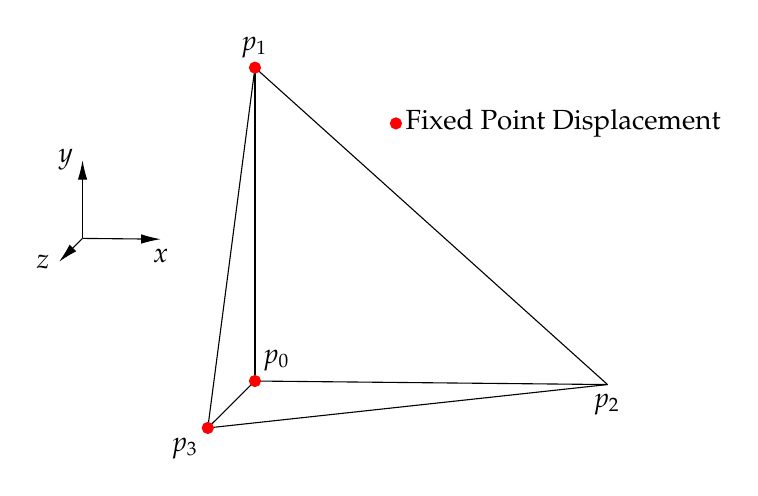
\begin{tikzpicture}
\draw[->] (-0.980017,2.03987) -- (0.0149875,2.0299);
\node[below] at (0.0149875,2.0299) {$x$};
\draw[->] (-0.980017,2.03987) -- (-0.980017,3.03487);
\node[left] at (-0.980017,3.03487) {$y$};
\draw[->] (-0.980017,2.03987) -- (-1.27952,1.74186);
\node[left] at (-1.27952,1.74186) {$z$};
\draw (1.20966,0.228594) -- (1.20966,4.20861);
\draw (1.20966,4.20861) -- (5.68718,0.183744);
\draw (5.68718,0.183744) -- (1.20966,0.228594);
\draw (0.610658,-0.367414) -- (1.20966,0.228594);
\draw (0.610658,-0.367414) -- (1.20966,4.20861);
\draw (0.610658,-0.367414) -- (5.68718,0.183744);
\draw[fill,red] (1.20966,0.228594) circle(0.07);
\node[above right] at (1.20966,0.228594) {$p_0$};
\draw[fill,red] (1.20966,4.20861) circle(0.07);
\node[above] at (1.20966,4.20861) {$p_1$};
\node[below] at (5.68718,0.183744) {$p_2$};
\draw[fill,red] (0.610658,-0.367414) circle(0.07);
\node[below left] at (0.610658,-0.367414) {$p_3$};
\draw[fill,red] (3,3.5) circle(0.07);
\node[right] at (3,3.5) {Fixed Point Displacement};
\end{tikzpicture}
\caption{Fixing Tetrahedron to the Wall}
\label{fig:fix:displacement}
\end{figure}

Consider linear equations with exactly one solution

\begin{equation}
a_1 x_0 + b_1 x_1 + c_1 x_2 = d_1
\end{equation}
\begin{equation}
a_2 x_0 + b_2 x_1 + c_2 x_2 = d_2
\end{equation}
\begin{equation}
a_3 x_0 + b_3 x_1 + c_3 x_2 = d_3
\end{equation}

or

\begin{equation}
\begin{bmatrix}
	a_1 & b_1 & c_1 \\
	a_2 & b_2 & c_2 \\
	a_3 & b_3 & c_3
\end{bmatrix}
\begin{bmatrix}
	x_0 \\
	x_1 \\
	x_2
\end{bmatrix}
=
\begin{bmatrix}
	d_1 \\
	d_2 \\
	d_3
\end{bmatrix}
\end{equation}

Fixing a point displacement requires setting selected variable to zero (no point displacement in this direction). Let's choose $x_1=0$. In order to preserve equality the constant $d_2$ must be freed. Disregarding zeros and moving new variable to the left side we obtain:

\begin{equation}
a_1 x_0 + c_1 x_2 = d_1
\end{equation}
\begin{equation}
a_2 x_0 + c_2 x_2 - d_2 = 0
\end{equation}
\begin{equation}
a_3 x_0 + c_3 x_2 = d_3
\end{equation}

\begin{equation}
\begin{bmatrix}
	a_1 & 0 & c_1 \\
	a_2 & -1 & c_2 \\
	a_3 & 0 & c_3
\end{bmatrix}
\begin{bmatrix}
	x_0 \\
	d_2 \\
	x_2
\end{bmatrix}
=
\begin{bmatrix}
	d_1 \\
	0 \\
	d_3
\end{bmatrix}
\end{equation}

Concluding - in order to fix some degrees of freedom the corresponding column of the stiffness matrix has to be zeroed and a fixed variable replaced with -1. Corresponding cell in solution vector will hold \textit{freed} constant.

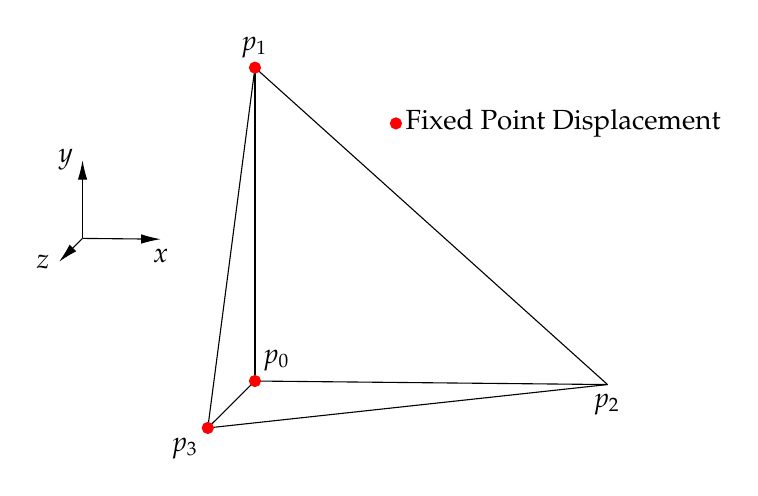
\begin{tikzpicture}
\draw[->] (-0.980017,2.03987) -- (0.0149875,2.0299);
\node[below] at (0.0149875,2.0299) {$x$};
\draw[->] (-0.980017,2.03987) -- (-0.980017,3.03487);
\node[left] at (-0.980017,3.03487) {$y$};
\draw[->] (-0.980017,2.03987) -- (-1.27952,1.74186);
\node[left] at (-1.27952,1.74186) {$z$};
\draw (1.20966,0.228594) -- (1.20966,4.20861);
\draw (1.20966,4.20861) -- (5.68718,0.183744);
\draw (5.68718,0.183744) -- (1.20966,0.228594);
\draw (0.610658,-0.367414) -- (1.20966,0.228594);
\draw (0.610658,-0.367414) -- (1.20966,4.20861);
\draw (0.610658,-0.367414) -- (5.68718,0.183744);
\draw[fill,red] (1.20966,0.228594) circle(0.07);
\node[above right] at (1.20966,0.228594) {$p_0$};
\draw[fill,red] (1.20966,4.20861) circle(0.07);
\node[above] at (1.20966,4.20861) {$p_1$};
\node[below] at (5.68718,0.183744) {$p_2$};
\draw[fill,red] (0.610658,-0.367414) circle(0.07);
\node[below left] at (0.610658,-0.367414) {$p_3$};
\draw[fill,red] (3,3.5) circle(0.07);
\node[right] at (3,3.5) {Fixed Point Displacement};
\end{tikzpicture}

\subsection{Implementation}

\lstinputlisting{populate.cpp}

\section{Solving Linear Equations by LU Decomposition Method}

\subsection{Explanation}

The method takes advantage of the fact that solving equation where matrix is triangular is straightforward. All cells above (or below) diagonal are equal zero and solution can be achieved in one iteration. The method at first breaks down the matrix into a multiplication of 2 triangular ones and then calculates sub-equations as follows.

\bigskip

Consider linear equations with exactly one solution

\begin{equation}
a_1 x_0 + b_1 x_1 + c_1 x_2 = d_1
\end{equation}
\begin{equation}
a_2 x_0 + b_2 x_1 + c_2 x_2 = d_2
\end{equation}
\begin{equation}
a_3 x_0 + b_3 x_1 + c_3 x_2 = d_3
\end{equation}

or

\begin{equation}
\begin{bmatrix}
	a_1 & b_1 & c_1 \\
	a_2 & b_2 & c_2 \\
	a_3 & b_3 & c_3
\end{bmatrix}
\begin{bmatrix}
	x_0 \\
	x_1 \\
	x_2
\end{bmatrix}
=
\begin{bmatrix}
	d_1 \\
	d_2 \\
	d_3
\end{bmatrix}
\end{equation}

\begin{equation}
\mathbf{K} \Delta \mathbf{P} = \mathbf{F}
\end{equation}

LU Decomposition Method is one of the simplest, though memory hungry solver. Let's decompose matrix $\mathbf{A}$ into 2 triangular matrices LU (lower and upper).

\begin{equation}
\begin{bmatrix}
	a_1 & b_1 & c_1 \\
	a_2 & b_2 & c_2 \\
	a_3 & b_3 & c_3
\end{bmatrix}
=
\begin{bmatrix}
	1 & 0 & 0 \\
	\color{green}{l_{21}} & 1 & 0 \\
	\color{green}{l_{31}} & \color{green}{l_{32}} & 1
\end{bmatrix}
\begin{bmatrix}
	\color{blue}{u_{11}} & \color{blue}{u_{12}} & \color{blue}{u_{13}} \\
	0 & \color{blue}{u_{22}} & \color{blue}{u_{23}} \\
	0 & 0 & \color{blue}{u_{33}}
\end{bmatrix}
\end{equation}

The equation can be rewritten as

\begin{equation}
\mathbf{LU} \Delta \mathbf{P} = \mathbf{F}
\end{equation}

When L and U are calculated the auxiliary vector Z can be simply solved

\begin{equation}
\mathbf{LZ} = \mathbf{F}
\end{equation}

Finally the vector $\Delta \mathbf{P}$ can be solved in similar way

\begin{equation}
\mathbf{U} \Delta \mathbf{P} = \mathbf{Z}
\end{equation}

\subsection{Solving an Example}

Let's solve a simple example.

\begin{equation}
\begin{bmatrix}
	1 & 2 & 3 \\
	4 & 14 & 19 \\
	5 & 58 & 80
\end{bmatrix}
\begin{bmatrix}
	x_0 \\
	x_1 \\
	x_2
\end{bmatrix}
=
\begin{bmatrix}
	10 \\
	59 \\
	211
\end{bmatrix}
\end{equation}

LU Decomposition

\begin{equation}
\begin{bmatrix}
	1 & 2 & 3 \\
	4 & 14 & 19 \\
	5 & 58 & 80
\end{bmatrix}
=
\begin{bmatrix}
	1 & 0 & 0 \\
	l_{21} & 1 & 0 \\
	l_{31} & l_{32} & 1
\end{bmatrix}
\begin{bmatrix}
	u_{11} & u_{12} & u_{13} \\
	0 & u_{22} & u_{23} \\
	0 & 0 & u_{33}
\end{bmatrix}
\end{equation}

It can be noticed that general direction of solving cells of matrices L and U is as depicted on figure \ref{fig:lu:direction}.

\begin{equation}
\begin{array}{lllll}
	1 = 1 * u_{11} & \Rightarrow & & \Rightarrow & \color{blue}{u_{11}} = 1 \\
	2 = 1 * u_{12} & \Rightarrow & & \Rightarrow & \color{blue}{u_{12}} = 2 \\
	3 = 1 * u_{13} & \Rightarrow & & \Rightarrow & \color{blue}{u_{13}} = 3 \\
	4 = l_{21}u_{11} & \Rightarrow & 4 = l_{21} * 1 & \Rightarrow & \color{green}{l_{21}} = 4 \\
	5 = l_{31}u_{11} & \Rightarrow & 5 = l_{31} * 1 & \Rightarrow & \color{green}{l_{31}} = 5 \\
	14 = l_{21}u_{12} + u_{22} & \Rightarrow & 14 = 4 * 2 + u_{22} & \Rightarrow & \color{blue}{u_{22}} = 6 \\
	19 = l_{21}u_{13} + u_{23} & \Rightarrow & 19 = 4 * 3 + u_{23} & \Rightarrow & \color{blue}{u_{23}} = 7 \\
	58 = l_{31}u_{12} + l_{32}u_{22} & \Rightarrow & 58 = 5 * 2 + l_{32} * 6 & \Rightarrow & \color{green}{l_{32}} = 8 \\
	80 = l_{31}u_{13} + l_{32}u_{23} + u_{33} & \Rightarrow & 80 = 5 * 3 + 8 * 7 + u_{33} & \Rightarrow & \color{blue}{u_{33}} = 9
\end{array}
\end{equation}

\begin{figure}[H]
\centering
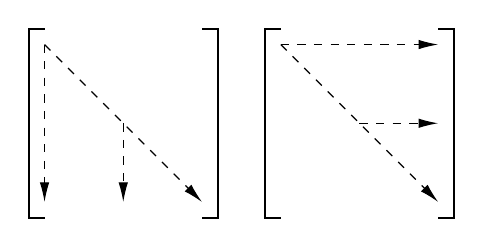
\begin{tikzpicture}
\draw[thick] (0,-0.2) -- (-0.2,-0.2) -- (-0.2,2.2) -- (0,2.2);
\draw[->,dashed] (0,2) -- (2,0);
\draw[->,dashed] (0,2) -- (0,0);
\draw[->,dashed] (1,1) -- (1,0);
\draw[thick] (2,-0.2) -- (2.2,-0.2) -- (2.2,2.2) -- (2,2.2);
\draw[thick] (3,-0.2) -- (2.8,-0.2) -- (2.8,2.2) -- (3,2.2);
\draw[->,dashed] (3,2) -- (5,0);
\draw[->,dashed] (3,2) -- (5,2);
\draw[->,dashed] (4,1) -- (5,1);
\draw[thick] (5,-0.2) -- (5.2,-0.2) -- (5.2,2.2) -- (5,2.2);
\end{tikzpicture}
\caption{Direction of the Decomposition in Matrices L and U}
\label{fig:lu:direction}
\end{figure}

Verification of LU Decomposition

\begin{equation}
\begin{bmatrix}
	1 & 2 & 3 \\
	4 & 14 & 19 \\
	5 & 58 & 80
\end{bmatrix}
=
\begin{bmatrix}
	1 & 0 & 0 \\
	4 & 1 & 0 \\
	5 & 8 & 1
\end{bmatrix}
\begin{bmatrix}
	1 & 2 & 3 \\
	0 & 6 & 7 \\
	0 & 0 & 9
\end{bmatrix}
\end{equation}

Solving the auxiliary Z vector

\begin{equation}
\begin{bmatrix}
	1 & 0 & 0 \\
	4 & 1 & 0 \\
	5 & 8 & 1
\end{bmatrix}
\begin{bmatrix}
	z_0 \\
	z_1 \\
	z_2
\end{bmatrix}
=
\begin{bmatrix}
	10 \\
	59 \\
	211
\end{bmatrix}
\end{equation}

\begin{equation}
\begin{array}{llllll}
	1 * z_0 = 10 & \Rightarrow & & \Rightarrow & z_0 = 10 \\
	4 * z_0 + 1 * z_1 = 59 & \Rightarrow & 4 * 10 + z_1 = 59 & \Rightarrow & z_1 = 19 \\
	5 * z_0 + 8 * z_1 + 1 * z_2 = 211 & \Rightarrow & 5 * 10 + 8 * 19 + 1 * z_2 = 211 & \Rightarrow & z_2 = 9
\end{array}
\end{equation}

Verification

\begin{equation}
\begin{bmatrix}
	1 & 0 & 0 \\
	4 & 1 & 0 \\
	5 & 8 & 1
\end{bmatrix}
\begin{bmatrix}
	10 \\
	19 \\
	9
\end{bmatrix}
=
\begin{bmatrix}
	10 \\
	59 \\
	211
\end{bmatrix}
\end{equation}

The final solution

\begin{equation}
\begin{bmatrix}
	1 & 2 & 3 \\
	0 & 6 & 7 \\
	0 & 0 & 9
\end{bmatrix}
\begin{bmatrix}
	x_0 \\
	x_1 \\
	x_2
\end{bmatrix}
=
\begin{bmatrix}
	10 \\
	19 \\
	9
\end{bmatrix}
\end{equation}

\begin{equation}
\begin{array}{llllll}
	9 * x_2 = 9 & \Rightarrow & & \Rightarrow & x_2 = 1 \\
	6 * x_1 + 7 * x_2 = 19 & \Rightarrow & 6 * x_1 + 7 * 1 = 19 & \Rightarrow & x_1 = 2 \\
	1 * x_0 + 2 * x_1 + 3 * x_2 = 10 & \Rightarrow & 1 * x_0 + 2 * 2 + 3 * 1 = 10 & \Rightarrow & x_0 = 3
\end{array}
\end{equation}

Verification

\begin{equation}
\begin{bmatrix}
	1 & 2 & 3 \\
	0 & 6 & 7 \\
	0 & 0 & 9
\end{bmatrix}
\begin{bmatrix}
	3 \\
	2 \\
	1
\end{bmatrix}
=
\begin{bmatrix}
	10 \\
	19 \\
	9
\end{bmatrix}
\end{equation}

Final verification of the original equation

\begin{equation}
\begin{bmatrix}
	1 & 2 & 3 \\
	4 & 14 & 19 \\
	5 & 58 & 80
\end{bmatrix}
\begin{bmatrix}
	3 \\
	2 \\
	1
\end{bmatrix}
=
\begin{bmatrix}
	10 \\
	59 \\
	211
\end{bmatrix}
\end{equation}

\subsection{Pitfalls of Direct Methods}

The present example uses LU Decomposition for solving matrix equations. The main downside of such approach is that data blocks are composed mostly with zeros. It is very inefficient management of memory and can be used only for simple geometries. Bigger examples may not fit into memory of modern computers.
More realistic model should be solved by one of sparse matrix methods. The most promising of them is Conjugate Gradient Method. Further work on next version of this document will be focused on it.

\subsection{The Concrete Example Result Presentation}

The below matrix equation presents the stiffness matrix, the displacement vector and external forces applied in selected points. Some cells where $-1$ is shown are used for fixed displacements and were chosen to compute reaction forces in corresponding displacement vector. The simplicity dictates such approach for price of loosing symmetry of matrix.

\bigskip

The data in the form

\begin{equation}
\mathbf{K} \Delta \mathbf{P} = \mathbf{F}
\end{equation}

is generated below as a result of computation of the main example

\begin{equation}
\resizebox{.93 \textwidth}{!} {$
\begin{bmatrix}
\color{blue}{-1} & . & . & . & . & . & -222.2 & . & . & . & . & . \\
. & 250 & . & . & -250 & . & . & . & . & . & . & . \\
. & . & \color{blue}{-1} & . & . & . & . & . & . & . & . & . \\
. & . & . & \color{blue}{-1} & -82.47 & . & -92.78 & 82.47 & . & . & . & . \\
. & -250 & . & . & 366 & . & 82.47 & -73.31 & . & . & . & . \\
. & . & . & . & -64 & \color{blue}{-1} & . & . & . & . & . & . \\
. & . & . & . & 82.47 & . & 363 & -82.47 & -64 & . & . & . \\
. & . & . & . & -73.31 & . & -82.47 & 73.31 & . & . & . & . \\
. & . & . & . & . & . & -64 & . & 85.33 & . & . & . \\
. & . & . & . & . & . & -48 & . & 64 & \color{blue}{-1} & . & . \\
. & . & . & . & -42.67 & . & . & . & . & . & \color{blue}{-1} & . \\
. & . & . & . & 64 & . & 64 & . & -85.33 & . & . & \color{blue}{-1}
\end{bmatrix}
\begin{bmatrix}
\color{blue}{-56.25} \\
0.7031 \\
. \\
\color{blue}{33.75} \\
0.7031 \\
\color{blue}{-45} \\
0.2531 \\
1.397 \\
0.5414 \\
\color{blue}{22.5} \\
\color{blue}{-30} \\
\color{blue}{15}
\end{bmatrix}=
\begin{bmatrix}
. \\
. \\
. \\
. \\
. \\
. \\
. \\
30 \\
30 \\
. \\
. \\
.
\end{bmatrix}
$}
\end{equation}

\subsection{Implementation of LU Decomposition Method}

\lstinputlisting{calculate.cpp}

\section{The 3D Data Presentation in the Documentation}

This chapter tries to explain how to present three-dimensional data in the document. Using only $x,y$ and removing $z$ coordinate is not a good solution since we loose part of the information and presented figures are not clear. Rotation is much better as all of original coordinates can be used and after transformation the new coordinate $z'$ can be discarded without loosing general understanding.

\subsection{Point Rotation}

Let's consider rotation of a point in coordinates x, y

\begin{figure}[H]
\centering
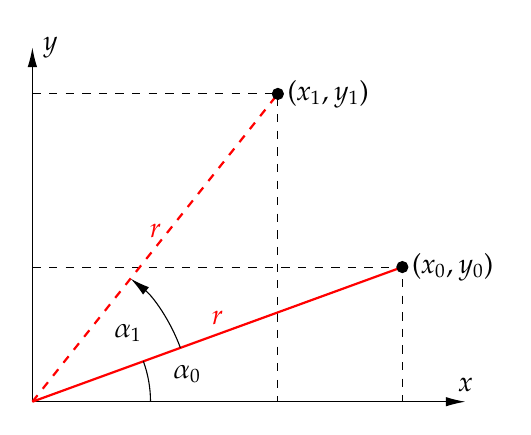
\begin{tikzpicture}
\draw[<->] (0,4.5) -- (0,0) -- (5.5,0);
\node[above] at (5.5,0) {$x$};
\node[right] at (0,4.5) {$y$};
\draw[dashed] (0,1.71005) -- (4.69848,1.71005) -- (4.69848,0);
\draw[dashed] (0,3.90907) -- (3.11755,3.90907) -- (3.11755,0);
\draw[thick,red] (0,0) -- (4.69848,1.71005);
\node[red,above] at (2.34924,0.855026) {$r$};
\node[right] at (4.69848,1.71005) {$(x_0,y_0)$};
\draw[fill] (4.69848,1.71005) circle(0.07);
\draw[thick,dashed,red] (0,0) -- (3.11755,3.90907);
\node[red,above] at (1.55878,1.95454) {$r$};
\node[right] at (3.11755,3.90907) {$(x_1,y_1)$};
\draw[fill] (3.11755,3.90907) circle(0.07);
\draw (1.5,0) arc (0:20:1.5);
\node at (1.96962,0.347286) {$\alpha_0$};
\draw[->] (1.87939,0.684021) arc (20:51.4286:2);
\node at (1.21792,0.875593) {$\alpha_1$};
\end{tikzpicture}
\caption{Point Rotation}
\label{fig:point:rotation}
\end{figure}

From geometry on the figure \ref{fig:point:rotation} we can obtain

\begin{equation}
x_0 = r \cos \alpha_0
\end{equation}
\begin{equation}
y_0 = r \sin \alpha_0
\end{equation}
\begin{equation}
x_1 = r \cos (\alpha_0 + \alpha_1) = r \cos \alpha_0 \cos \alpha_1 - r \sin \alpha_0 \sin \alpha_1
\end{equation}
\begin{equation}
y_1 = r \sin (\alpha_0 + \alpha_1) = r \sin \alpha_0 \cos \alpha_1 + r \cos \alpha_0 \sin \alpha_1
\end{equation}

hence

\begin{equation}
x_1 = x_0 \cos \alpha_1 - y_0 \sin \alpha_1
\end{equation}
\begin{equation}
y_1 = x_0 \sin \alpha_1 + y_0 \cos \alpha_1
\end{equation}

Changes on the axis z can be expressed simply by $z_1 = z_0$. Constructing three-dimensional matrix we obtain rotation operator around the axis z

\begin{equation}
\begin{bmatrix}
	x_1 \\
	y_1 \\
	z_1
\end{bmatrix}
=
\begin{bmatrix}
	\cos \alpha_1 & - \sin \alpha_1 & 0 \\
	\sin \alpha_1 & \cos \alpha_1 & 0 \\
	0 & 0 & 1
\end{bmatrix}
\begin{bmatrix}
	x_0 \\
	y_0 \\
	z_0
\end{bmatrix}
\end{equation}

\begin{equation}
\mathbf{P_1} = \mathbf{R_z P_0}
\end{equation}

\subsection{An Example of Rotated Tetrahedron}

The example rotates all points of geometry around the axis y and then x. It can be expressed as

\begin{equation}
\mathbf{P_1} = \mathbf{R_x R_y P_0}
\end{equation}

In details

\begin{equation}
\begin{bmatrix}
	x_1 \\
	y_1 \\
	z_1
\end{bmatrix}
=
\begin{bmatrix}
	1 & 0 & 0 \\
	0 & c_x & -s_x \\
	0 & s_x & c_x
\end{bmatrix}
\begin{bmatrix}
	c_y & 0 & -s_y \\
	0 & 1 & 0 \\
	s_y & 0 & c_y
\end{bmatrix}
\end{equation}

\begin{equation}
\begin{bmatrix}
	x_1 \\
	y_1 \\
	z_1
\end{bmatrix}
=
\begin{bmatrix}
	c_y & 0 & -s_y \\
	-s_xs_y & c_x & -s_xc_y \\
	c_xs_y & s_x & c_xc_y
\end{bmatrix}
\begin{bmatrix}
	x_0 \\
	y_0 \\
	z_0
\end{bmatrix}
\end{equation}

Finally the coordinate $z_1$ is cut off as it does not have representation in 2D. Visualized results are presented on the figure \ref{fig:object:rotation}.

\begin{figure}[H]
\centering
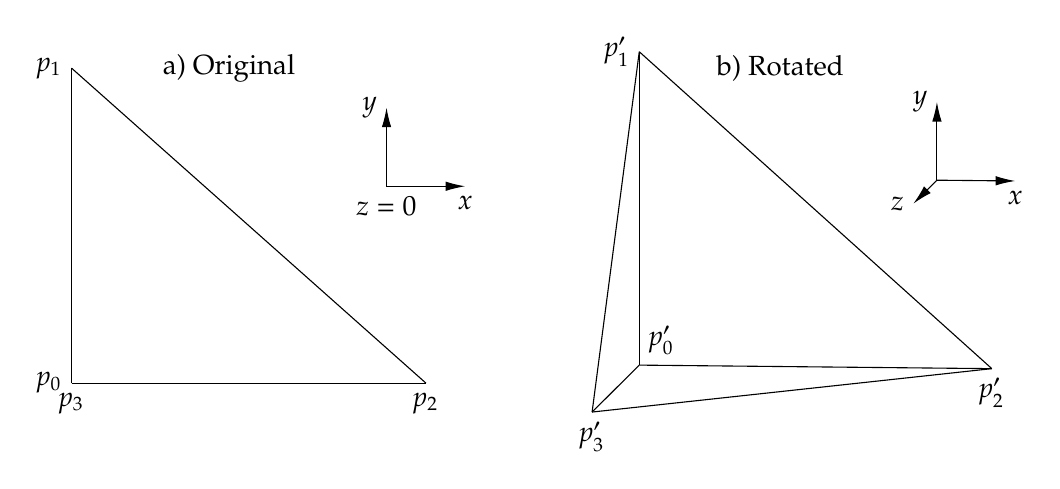
\begin{tikzpicture}
\node at (-4,4) {a) Original};
\draw[<->] (-2,3.5) -- (-2,2.5) -- (-1,2.5);
\node[left] at (-2,3.5) {$y$};
\node[below] at (-2,2.5) {$z=0$};
\node[below] at (-1,2.5) {$x$};
\draw (-6,0) -- (-6,4);
\draw (-6,4) -- (-1.5,0);
\draw (-1.5,0) -- (-6,0);
\draw (-6,0) -- (-6,0);
\draw (-6,0) -- (-6,4);
\draw (-6,0) -- (-1.5,0);
\node[left] at (-6,0) {$p_0$};
\node[left] at (-6,4) {$p_1$};
\node[below] at (-1.5,0) {$p_2$};
\node[below] at (-6,0) {$p_3$};
\node at (3,4) {b) Rotated};
\draw[->] (4.99001,2.57707) -- (5.98501,2.5671);
\node[below] at (5.98501,2.5671) {$x$};
\draw[->] (4.99001,2.57707) -- (4.99001,3.57207);
\node[left] at (4.99001,3.57207) {$y$};
\draw[->] (4.99001,2.57707) -- (4.69051,2.27907);
\node[left] at (4.69051,2.27907) {$z$};
\draw (1.20966,0.228594) -- (1.20966,4.20861);
\draw (1.20966,4.20861) -- (5.68718,0.183744);
\draw (5.68718,0.183744) -- (1.20966,0.228594);
\draw (0.610658,-0.367414) -- (1.20966,0.228594);
\draw (0.610658,-0.367414) -- (1.20966,4.20861);
\draw (0.610658,-0.367414) -- (5.68718,0.183744);
\node[above right] at (1.20966,0.228594) {$p_0'$};
\node[left] at (1.20966,4.20861) {$p_1'$};
\node[below] at (5.68718,0.183744) {$p_2'$};
\node[below] at (0.610658,-0.367414) {$p_3'$};
\end{tikzpicture}
\caption{Original and Rotated Tetrahedron Example}
\label{fig:object:rotation}
\end{figure}

\subsection{Implementation of the Rotation Procedure}

\lstinputlisting{rotate.cpp}

\section{Summary}

Finally the article described all practical aspects of the finite method presentation. Starting with geometry definition, theoretical method explanation, solving matrix equations and 3D data presentation. Reader could confront mathematical aspects with practical implementation for better understanding.

\end{document}
